\section{Численные алгоритмы минимизации функционалов}\label{sec:ch4/sec2}
В данной главе мы опишем градиентный спуск и его модификации,
а также некоторые стохастические методы.

\subsection{Градиентный спуск и модификации}
\label{subsec:ch4/sec2/grad}
\textit{Градиентный спуск} - это способ минимизации целевой функции
$J(\boldsymbol{\theta})$, параметризованной параметрами модели
$\boldsymbol{\theta} \in \mathbb{R}^{d}$, путем обновления параметров
в направлении, противоположном градиенту целевой функции
$\nabla_{\boldsymbol{\theta}} J(\boldsymbol{\theta})$
относительно параметров.
Скорость обучения $\eta$ определяет размер шагов, которые мы делаем,
чтобы достичь (локального) минимума.
Иными словами, мы следуем направлению наклона поверхности,
созданной целевой функцией, вниз до тех пор,
пока не достигнем локального минимума.

Известны различные способы модификации градиентного спуска.
Перечислим некоторые из них.

\textbf{Градиентный спуск с проекцией}

Метод градиентного спуска широко используется для минимизации дифференцируемой
функции $f(\mathbf{x})$, итеративно двигаясь в направлении наибольшего убывания.
Алгоритм осуществляется путем обновления параметров
$\mathbf{x} \in \mathbb{R}^n$ в направлении, противоположном
градиенту функции $\nabla f(\mathbf{x})$ с величиной шага
(скорость обучения) $\eta$.
Этот простой, но мощный алгоритм оптимизации используется во
множестве приложений, таких как машинное обучение, компьютерное
зрение и обработка сигналов.
В некоторых случаях задача оптимизации
имеет дополнительные ограничения, которые могут быть включены в
алгоритм градиентного спуска с использованием проекции.
В этом отчете представлен обзор метода градиентного спуска с проекцией,
а также обсуждаются его основные особенности и приложения.


Цель алгоритма градиентного спуска - минимизировать функцию
$f(\mathbf{x})$, итеративно обновляя параметры следующим образом:

\[ x_{k+1} = x_k - \eta \nabla f(x_k), \]

где $\mathbf{x}_k$ - вектор параметров на итерации $k$,
$\eta$ - величина шага, и $\nabla f(\mathbf{x}_k)$ - градиент
функции на итерации $k$.
Когда задача оптимизации включает ограничения, алгоритм
градиентного спуска должен быть изменен, чтобы учесть эти ограничения.
Один из распространенных подходов состоит в использовании проекции
на множество ограничений.


Пусть $\mathcal{C}$ - множество ограничений.
Алгоритм градиентного спуска с проекцией
можно описать следующим образом:
\[ x_{k+1} = \mathcal{P}_{\mathcal{C}}(x_k - \eta \nabla f(x_k)), \]

где $\mathcal{P}_{\mathcal{C}}(\cdot)$ - оператор проекции
на множество ограничений $\mathcal{C}$.
Проекция обеспечивает сохранение обновленного
вектора параметров $\mathbf{x}_{k+1}$ в пределах множества
ограничений, таким образом, удовлетворяя ограничения задачи.

\textbf{Оператор проекции}
Оператор проекции $\mathcal{P}_{\mathcal{C}}(\cdot)$
проецирует заданную точку на множество ограничений $\mathcal{C}$.
Проекция точки $\mathbf{y}$ на множество $\mathcal{C}$ определяется как:
\[
    \mathcal{P}_{\mathcal{C}}(y) =
    \arg \min_{x \in \mathcal{C}} \|y - x\|^2,
\]

где $\|\cdot\|$ обозначает евклидову норму.
Оператор проекции находит точку в множестве ограничений
$\mathcal{C}$, которая ближе всего к заданной точке $\mathbf{y}$.

\textbf{Примеры множеств ограничений}

Множество ограничений может иметь различные формы
в зависимости от задачи оптимизации.
Некоторые распространенные множества ограничений включают:
\begin{itemize}
    \item \textbf{Ограничения-коробки:} Множество ограничений представляет
    собой коробку, определенную как
    $\mathcal{C} = \{\mathbf{x} \in \mathbb{R}^n , | , a_i
    \leq x_i \leq b_i, , i=1,\dots,n\}$.
    В этом случае оператор проекции можно вычислить поэлементно:
    \[
        (\mathcal{P}_{\mathcal{C}}(y))_i =
        \min(\max(y_i, a_i), b_i), \quad i=1,\dots,n.
    \]

    \item \textbf{Ограничения-шары:} Множество ограничений представляет
    собой закрытый шар с радиусом $r$ и центром $\mathbf{c}$,
    определенный как $\mathcal{C} = \{\mathbf{x} \in \mathbb{R}^n , | ,
    \|\mathbf{x} - \mathbf{c}\| \leq r\}$.
    Оператор проекции для этого множества ограничений:
    \[
        \mathcal{P}_{\mathcal{C}}(y) = c
        + \min\left(1, \frac{r}{\|y-c\|}\right)(y-c).
    \]
    \item \textbf{Ограничения-симплексы:} Множество ограничений
    представляет собой симплекс, определенный как
    $\mathcal{C} = \{\mathbf{x} \in \mathbb{R}^n ,
    | , \mathbf{x} \geq \mathbf{0}, , \sum_{i=1}^n x_i = 1\}$.
    Оператор проекции для этого множества ограничений включает
    более сложный алгоритм, такой как тот,
    который представлен, например~\cite{Duchi2011}.
\end{itemize}

Градиентный спуск с проекцией нашел различные применения
в разных областях, включая:

\begin{itemize}
    \item \textbf{Разреженная оптимизация:}
    В машинном обучении разреженность является желаемым
    свойством для интерпретируемости модели и отбора признаков.
    Добавление ограничения $\ell_1$ к задаче оптимизации
    обеспечивает разреженность решения.
    Алгоритм градиентного спуска с проекцией может
    быть использован для решения таких задач.

    \item \textbf{Обработка изображений:} В обработке изображений
    минимизация полной вариации является популярным подходом
    для устранения шума и восстановления изображений.
    Задача оптимизации заключается в минимизации негладкой целевой
    функции с ограничениями на изображение.
    Градиентный спуск с проекцией может быть
    использован для решения этих типов задач.

    \item \textbf{Сжатое ощущение:} Сжатое ощущение
    (Compressed Sensing) - это метод, используемый в обработке
    сигналов для восстановления разреженного сигнала из
    небольшого количества линейных измерений.
    Задача восстановления формулируется как задача оптимизации
    с ограничениями на разреженность.
    Градиентный спуск с проекцией может быть использован для
    решения задачи восстановления сжатого ощущения.
\end{itemize}

Градиентный спуск с проекцией является универсальным алгоритмом
оптимизации, который позволяет включать ограничения в
стандартный метод градиентного спуска.
Оператор проекции обеспечивает выполнение
ограничений задачи при обновлении параметров.
Алгоритм успешно применяется в различных областях, таких как
машинное обучение, обработка изображений и обработка сигналов.


\textbf{Момент}
Градиентный спуск испытывает трудности при навигации в оврагах,
то есть в областях, где поверхность круче изгибается в одном измерении,
чем в другом~\cite{Sutton1986},
что обычно встречается в окрестности локальных оптимумов.
В таких сценариях SGD колеблется по склонам оврага,
делая только неуверенный
прогресс вдоль дна к локальному оптимуму, как на изображении~\ref{fig:momentums}.

\begin{figure}[ht]
    \begin{minipage}[b][][b]{0.49\linewidth}\centering
        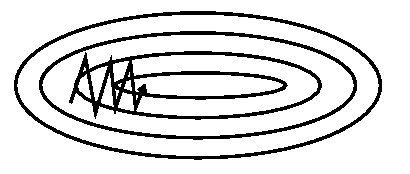
\includegraphics[width=1\linewidth]{4_2/without_momentum} \\ а) SGD без момента
    \end{minipage}
    \hfill
    \begin{minipage}[b][][b]{0.49\linewidth}\centering
        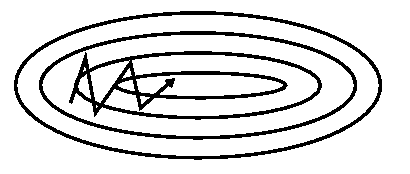
\includegraphics[width=1\linewidth]{4_2/with_momentum} \\ б) SGD с моментом
    \end{minipage}
    \caption{Результаты второго эксперимента}\label{fig:momentums}
\end{figure}

Метод момента~\cite{QIAN1999145} помогает ускорить
SGD в соответствующем направлении
и сглаживает колебания.
Он делает это, добавляя долю $\gamma$ вектора обновления прошлого
временного шага к текущему вектору обновления:

\begin{equation*}
    v_t = \gamma v_{t-1} + \eta \nabla_{\theta} J(\theta)
\end{equation*}

\begin{equation*}
    \theta = \theta - v_t
\end{equation*}

Примечание: Некоторые реализации меняют знаки в уравнениях.
Обычно момент инерции $\gamma$ устанавливается равным 0.9
или близким к этому значению.

По сути, при использовании момента мы толкаем шар вниз по склону.
Шар накапливает момент, катаясь вниз по склону,
становясь все быстрее и быстрее по пути
(пока не достигнет своей предельной скорости,
если есть сопротивление воздуха, то есть $\gamma < 1$).
То же самое происходит с нашими обновлениями параметров:
момент увеличивается для измерений, чьи градиенты указывают
в одном направлении, и уменьшает обновления для измерений,
чьи градиенты меняют направления.
В результате мы получаем более быстрое
сходимости и уменьшение колебаний.

\textbf{Ускоренный градиент Нестерова}

Однако шар, который катится вниз по склону, слепо следуя склону,
является крайне неудовлетворительным.
Мы хотели бы иметь более умный шар, шар, который имеет
представление о том, куда он движется, так что он знает,
когда нужно замедлиться перед тем, как склон вновь поднимется.

Мы знаем, что мы будем использовать наш момент
$\gamma v_{t-1}$ для перемещения параметров $\theta$.
Вычисление $\theta - \gamma v_{t-1}$ дает нам приближение
следующей позиции параметров
(градиент отсутствует для полного обновления),
грубое представление о том, куда будут двигаться наши параметры.
Теперь мы можем фактически заглянуть вперед,
рассчитывая градиент не относительно наших текущих параметров
$\theta$, но относительно приблизительного
будущего положения наших параметров:

\begin{equation*}
    v_t = \gamma v_{t-1} + \eta \nabla_{\theta} J(\theta - \gamma v_{t-1})
\end{equation*}

\begin{equation*}
    \theta = \theta - v_t
\end{equation*}

Опять же, мы устанавливаем момент $\gamma$ равным значению около 0.9.
В то время как момент сначала вычисляет текущий
градиент (небольшой синий вектор на изображении 4),
а затем делает большой скачок в направлении обновленного
накопленного градиента (большой синий вектор), NAG сначала делает
большой скачок в направлении предыдущего накопленного градиента
(коричневый вектор), измеряет градиент и затем делает корректировку
(красный вектор), что приводит к полному обновлению NAG (зеленый вектор).
\begin{figure}[ht]
    \centerfloat{ 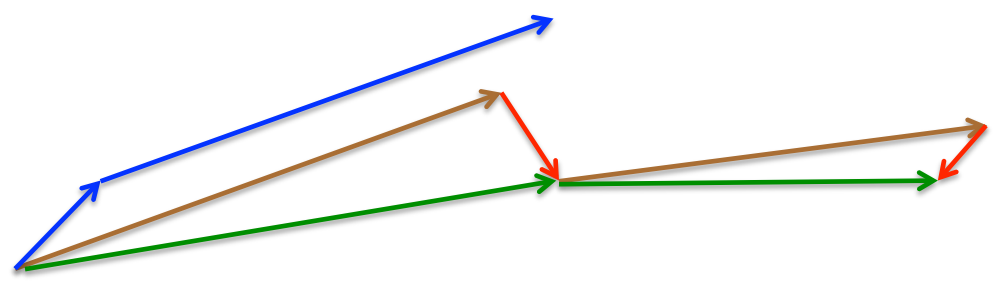
\includegraphics[scale=0.5]{4_2/nesterov_update_vector} }
    \caption{Обновление Нестерова (Source: G. Hinton's lecture 6c)}\label{fig:4_2:1}
\end{figure}

Более подробный разбор механики градиента Нестерова
можно найти в~\cite{Sutskever2013}.

Теперь, когда мы можем адаптировать наши обновления к наклону
нашей функции ошибок и ускорять SGD, мы также хотели бы адаптировать
наши обновления к каждому отдельному параметру, чтобы выполнять
большие или меньшие обновления в зависимости от их важности.

\subsection{Метод роя частиц}\label{subsec:ch4/sec2/stokhastic}
Оптимизация на основе роя частиц (PSO) - популярный алгоритм метаэвристической
оптимизации, вдохновленный природой, предложенный Кеннеди и Эберхартом
в 1995 году~\cite{kennedy1995}.
Он вдохновлен социальным поведением стай птиц и косяков рыб.
PSO широко применяется для решения различных задач оптимизации благодаря
своей простоте, легкой реализации и быстрой сходимости.


\textbf{Алгоритм оптимизации на основе роя частиц}
Алгоритм PSO состоит из роя частиц, каждая из которых представляет собой
потенциальное решение задачи оптимизации.
Частицы перемещаются по пространству поиска, корректируя свои позиции
на основе своего собственного опыта и опыта своих соседей с целью найти
глобальный минимум или максимум целевой функции.
В качестве примера применения данного метода приведём~\cite{Alekseev2019Simulation},
в которой задача управления решается методом роя частиц.

\textbf{Представление частиц и инициализация}

Частица роя представляется вектором своего положения
$\mathbf{x}i = (x{i1}, x_{i2}, \dots, x_{id})^T$ и вектором скорости
$\mathbf{v}i = (v{i1}, v_{i2}, \dots, v_{id})^T$,
где $d$ - размерность пространства поиска.
Рой инициализируется с $N$ частицами, и их начальные положения
и скорости обычно случайным образом генерируются в пределах
границ пространства поиска.

\textbf{Правила обновления частиц}

На каждой итерации частицы обновляют свои скорости и положения в
соответствии с следующими правилами:

\begin{equation*}
    \mathbf{v}{i}(t+1) = \omega \mathbf{v}{i}(t)
    + c_1 r_1 (\mathbf{p}{i} - \mathbf{x}{i}(t))
    + c_2 r_2 (\mathbf{p}{g} - \mathbf{x}{i}(t))
\end{equation*}

\begin{equation*}
    \mathbf{x}{i}(t+1) = \mathbf{x}{i}(t) + \mathbf{v}_{i}(t+1)
\end{equation*}

где:
\begin{itemize}
    \item $t$ - текущая итерация,
    \item $\omega$ - вес инерции, который балансирует глобальные и локальные возможности поиска,
    \item $c_1$ и $c_2$ - когнитивные и социальные коэффициенты ускорения соответственно,
    \item $r_1$ и $r_2$ - случайные числа, равномерно распределенные в интервале $[0, 1]$,
    \item $\mathbf{p}_i$ - лучшее личное положение, найденное частицей $i$,
    \item $\mathbf{p}_g$ - лучшее глобальное положение, найденное всем роем.
\end{itemize}

Вес инерции $\omega$ может быть как постоянным, так и
адаптивно корректироваться в процессе оптимизации.
Общий подход к адаптивной корректировке - использование
линейно убывающего веса инерции:

\begin{equation*}
    \omega(t) = \omega_{\max} - \frac{t(\omega_{\max}
        - \omega_{\min})}{T}
\end{equation*}

где $T$ - максимальное число итераций, а $\omega_{\max}$
и $\omega_{\min}$ - максимальное и
минимальное значения веса инерции соответственно.

\textbf{Критерии завершения}

Алгоритм PSO обычно завершается, когда выполняется одно из следующих условий:

\begin{enumerate}
    \item Достигнуто максимальное количество итераций.
    \item Глобальное лучшее значение приспособленности не улучшается
    значительно в течение предопределенного числа последовательных итераций.
    \item Глобальное лучшее значение приспособленности
    достигает предопределенного приемлемого порога.
\end{enumerate}

\textbf{Применение алгоритма оптимизации роем частиц}

Алгоритм PSO был применен к широкому спектру задач оптимизации, включая:

\begin{itemize}
    \item Оптимизация функций: PSO может быть использован для поиска
    глобального минимума или максимума сложных функций
    с несколькими переменными и ограничениями.
    \item Машинное обучение и интеллектуальный анализ данных:
    PSO применялся для выбора признаков, кластеризации и настройки
    параметров различных алгоритмов машинного обучения.
    \item Комбинаторная оптимизация: PSO был адаптирован для решения задач,
    таких как задача коммивояжера, задачи расписания
    и задачи маршрутизации транспортных средств.
    \item Инженерный дизайн: PSO используется для оптимизации различных
    инженерных задач, таких как дизайн антенн,
    структурный дизайн и системы управления.
\end{itemize}

\textbf{Заключение}
Метод роя частиц — это мощный алгоритм оптимизации,
основанный на социальном поведении птичьих стай и косяков рыб.
Его простота, легкая реализация и быстрая сходимость делают его
привлекательным выбором для решения различных задач оптимизации.
Алгоритм успешно применяется в различных областях, включая
оптимизацию функций, машинное обучение,
комбинаторную оптимизацию и инженерное проектирование.
